\documentclass{article}
\usepackage{graphicx} % Required for inserting images
\usepackage{amsmath}
\usepackage{algorithm}
\usepackage{algpseudocode}
\usepackage{mathrsfs}
\usepackage{array} % For better table alignment
\usepackage{booktabs}
\usepackage{multirow} % For multi-row cells

\title{Comparison of Frank-Wolfe Variants for White-Box Adversarial Attacks}
\author{Tanner Aaron Graves - 2073559\and Alessandro Pala - 2107800}
\date{June 2024}

\begin{document}

\maketitle 
\section{Abstract}
With deep neural networks becoming ubiquitous in application, adversarial attacks have received much attention, as it has proved remarkably easy to create adversarial examples- genuine data that undergoes a minimal and unobtrusive corruption process in order to maximally harm the performance of a model. Access to a models architecture can enable white-box attacks, where gradients of loss with respect to input examples are exploited to create adversarial examples. The requirement that examples be minimally perturbed is a constraint on the optimization. The ability of Frank-wolf and variants have gathered much attention for their ability to be efficiently create adversarial examples while staying in a constraint set. In the paper we introduce discuss the application of Frank-Wolfe and two variants to this non-convex constrained optimization problem. Furthermore we discuss popular optimizations and their effect convergence and attack efficacy, comparing performance on attacks on models trained on MNSIT, FashionMNIST, and CFAIR-10 datasets. Finally, there is a discussion of the theoretical underpinnings of each algorithm. 

\section{Introduction}
Adversarial attacks on CNNs are often stated as the following constrained optimization problem:
\begin{equation}
\begin{aligned}
\min_x \quad & f(x)\\
\text{s.t.} \quad & ||x||_p \leq \epsilon
\end{aligned}
\end{equation}
% targeted / untargeted
In the case of untargeted attacks on a classifier, we perturb an example with the aim it be incorrectly predicted as any other class. Here $f(x)$ is the loss function of the attacked model $-\ell(x, \hat{y})$. In the case of targeted attacks, we aim to maximize the likelihood of another class $y \neq \hat{y}$. The cost then is $f(x) = \ell(x, y)$. We have implemented both targeted and untargeted attacks, and come to focus on targeted attacks as the algorithms are seen to require more iterations to converge. 
%constraint set
The $L_p$ constraint $||x||_p \leq \epsilon$ directly restricts the size of perturbations made the to the example. An inherent problem of DNNs is often attacks can be consistently successful even with very small, even imperceptible $\epsilon$. Different choices of $p$ may be made giving $||x||_p = (\sum_i{x_i^p})^{1/p}$. We have implemented and provide results for the $L_2$ and the $L_\infty(x) = \max_i |x_i|$ norms, focusing mostly on the ladder. 
We define the constraint set $\mathcal{M} = \{x : L_p(x) \leq \epsilon\}$. 
Of particular note is when $\mathcal{M}$ is a polytope, as is the case when $p \in \{1, \infty\}$. This corresponds to models making perturbations that are either sparse or have a maximal disturbance along each element. In these cases, the constraint set can be expressed as the convex combination of a finite set of vertices $\mathcal{M} = \text{Conv}\{\mathcal{A}\}$. This will be of particular relevance in the discussion of Away-step and pairwise variants. Otherwise, $\mathcal{A}$ is taken to be the boundary of $\mathcal{M}$.\break
%Why is constraints an issue
The constrained nature of this problem limits the applicability of a method like gradient descent, and requires integrating knowledge of the constraint space for effective optimization. Methods like Fast Signed Gradient attacks and projected gradient descent are popular choices, but either create unsophisticated adversarial examples or require wasteful projection onto the constraint space. 

% LMO
We explore Frank-Wolfe variants which are well suited to this problem by ensuring feasibility within the constraint set at each iteration with the efficient solving of a Linear Minimization Oracle (LMO). 
$$
LMO_\mathcal{A}(\nabla f(x_t)) \in \arg \min_{x \in \mathcal{A}} \langle \nabla f(x_t), x\rangle
$$
The LMO is responsible for solving what is called the "Frank-Wolfe Subproblem" and at each iteration provides and optimal $s_t$ such that updating $x_{t+1}$ to move in the direction of $s_t$ will remain in $\mathcal{M}$ Given it moves no more than some maximum step-size. By solving the LMO efficiently, the algorithm ensures that each iteration makes significant progress towards the optimal solution while respecting the constraints, thereby maintaining feasibility and accelerating convergence. 
% LMO colsed form solutions
Efficient solving of the LMO requires exploiting the structure of the constraint set $\mathcal{M}$. In the case of the $L_\infty$ norm it has closed form solution:
$$LMO_\mathcal{A} = s_t = -\epsilon \, \text{sign}(\nabla f(x_t)) + x_0$$
%But can be given generally for any choice of $p \in [1, \infty]$.
%$$LMO_\mathcal{A}_i = -\epsilon \text{sign}(\nabla f(x_t))$$
%LMO complexity - FW.pdf
This is clearly of $O(n)$ complexity where $n$ is the number of elements in the gradient. This can be interpreted as defining an attack direction where each element is the maximum allowable perturbation $\pm \epsilon$ according to the gradient. With one iteration, this is exactly the outcome of a Fast Signed Gradient Attack. At each iteration, we can see that the LMO will give a vertex on the boundary of the constraint set $\mathcal{M}$ which was optimally chosen to be as close to the true gradient as possible while permitting subsequent iterations stay within the feasible set.


% FW GAP as Convergence Criterion
The constrained nature of the Adversarial Attack problem means that the norm of the gradient $||\nabla_x f(x)||$ is not a suitable convergence criterion, as boundary points need not have zero gradient. Instead, we adopt the Frank-Wolfe gap as a measure of both optimality and point feasibility. In the convex case, this gap measures the maximum improvement over the current iteration $x_t$ within the constraints $\mathcal{M}$ and is defined as:
$$g_t^{\text{FW}} := \max_{s \in \mathcal{M}} \langle x_t - s, \nabla f(x_t) \rangle = \langle -\nabla f(x_t), d_t^{\text{FW}} \rangle$$
The Frank-Wolfe gap $g_t^{\text{FW}}$ is always non-negative $g_t^{\text{FW}} \geq 0$ and is zero if and only if $x_t$ is a stationary point. This makes it a useful convergence criterion, particularly since stationary points need not have zero gradients in constrained problems. We found that $g_t^\text{FW} < 0.1$ to be a good convergence criterion for our models. In most circumstances, seccessful attacks will happen before this threashold. However, setting it higher seems to adversly effect attack success rate, and setting it lower is seen to require many more unneeded iterations. We cap the maximum iterations at $20$ in this work.

The loss functions of Deep Neural Networks (DNNs), which are commonly the subject of adversarial attacks, are highly non-convex. Thus, the convergence of Frank-Wolfe methods in these applications is complicated by the fact that we are not guaranteed to find a global optimum or a successful attack, but rather convergence to a stationary point. 
It is also worth noting that, in the context of adversarial attacks, the Frank-Wolfe gap serves as an imprecise surrogate for success. In many cases, Frank-Wolfe methods generate successful attacks several iterations before convergence. This is because achieving an incorrect class probability higher than the correct class is often sufficient for a successful attack, whereas convergence indicates the new output class probability has been maximized.

\section{Algorithms}
We implement the original FW algorithm and amodified version with momentum FW with momentum \cite{attacks}. We then compare the performance of these models with 2 variants \cite{fw-variants}: Away Step Frank Wolfe, and Pairwise Frank Wolfe by measuring attack success rate and average iterations required for convergence.

\subsection{Frank-Wolfe}
\begin{algorithm}
\caption{FW for adversarial attacks}\label{alg:cap}
\begin{algorithmic}[1]
\Require maximum iterations $T$, step-sizes $\{\gamma_t\}$, convergence tolerance $\delta$
\Ensure $y = x^n$
\State $x_0 = x_{\text{ori}}$
\For{$t = 1,...,T$}
	% for the sets use the notation from FW_varients for consistency
	% M is the condstrained space of the attack and A is the set of vertieces
	\State $s_t = {\arg \min}_{x\in\mathcal{M}} \langle x, \nabla f(x_t)\rangle$ \Comment{LMO step}
	\State $d_t = s_t - x_t$
	\State $x_{t+1} = x_t + \gamma_t d_t$
	% TODO: maybe mention FW gap converg crit here
	\If{$\langle d_t, -\nabla f(x)\rangle < \delta$} \text{return} \hfill \Comment{FW gap convergence criterion}
	\EndIf
\EndFor
\end{algorithmic}
\end{algorithm}

Observing oscillation in Frank Wolfe convergence is common and consequence of optimal points lying on a face of $\mathcal{M}$. Since at each iteration the method is moving towards a vertex of polytope $\mathcal{M}$, in $\mathcal{S}$, the method "zigzags", moving towards different points in effort to gradually approach the face on which the optimum lies. In the convex case, Frank Wolfe is seen to have linear complexity when optimal point $x^*$ lies in the interior of $\mathcal{M}$, the oscillation causes sub-linear convergence when $x^*$ on the boundary.
%citation needed
 We implement variants that aim to address this problem to provide better convergence. The simplest of which is adding momentum to standard frank wolf which replaces the gradient in the LMO calculation in line $(4)$ with a momentum term $m_t  = \beta m_{t-1} + (1-\beta) \nabla f(x_t)$ and initialize $m_0 = \nabla f(x_0)$. By considering this exponentially weighted average of gradient information, momentum variants are empirically observed to have nicer convergence. 

The FW algorithm has a useful interpretation that serves as basis for the following variants: Away-Step FW and Pairwise FW. Namely that at each iteration $x_t$ is perturbed in some direction $s_t$, making $x_{t+1}$ a convex combination of $x_t$ and $s_t$. We record these directions in an active set $S_{t+1} = S_t \bigcup \{s_t\}$ and observe that initially $x_0$ is a convex combination of of active set $S_0 = \{x_0\}$. Then by induction, $x_t$ is a convex combination of directions in $S_t$, admitting coefficients $\alpha$ such that $x_t = \sum_{s \in S_t} \alpha_{s} s$.
Each iteration of the FW algorithm is seen to increase or introduce the contribution of $s_t$ in the convex combination while shrink the $\alpha$ coefficients of all other vertices, or atoms uniformly.
The innovation of the Away-Step and Pairwise variant is to recognize contribution of "bad atoms" can prevent convergence to an optimum on the boundary. These variants more directly diminish such atoms contributions by either taking steps away from selected atoms, or transferring mass between two selected atoms at each iteration as the case with the pairwise variant.

\subsection{Away-Step Frank-Wolfe}
The away-step FW algorithm (AFW) defines a gap in two possible directions: the typical FW step $d_t^\text{FW}$ and an away direction $d_t^\text{A} = x_t - v_t$ where $v_t  \in {\arg \max}_{v\in S_t} \langle v, \nabla f(x_t)\rangle$. By comparing the gaps associated with the two directions, the algorithm compares the cost of taking a typical FW step to the cost associated with moving away from active atoms in $S_t$. Should this gap be less than that of moving towards the Frank Wolfe direction, the influence of the selected away atom $v_t\in S_t$ will be diminished, and even dropped if the corresponding $\alpha_{v_t} \leq 0$. 
The $\alpha$ updates can be seen to be inverse for that of a normal FW step. Here influence of $v_t$ is distributed uniformly to other active atoms. New coefficients for the convex combination are for $v_t$, $\alpha_{v_{t}} := (1+\gamma_t)\alpha_{v_t} - \gamma_t$, and otherwise $\alpha_{v_{t+1}} := (1+\gamma_t)\alpha_{v}$. 
The algorithm enables a "drop step" where the contribution of an atom is completely removed from the convex combination, alleviating the problem of oscillation when converging to an optimum on the boundary. 
This algorithm is proved to have linear convergence for convex problems
\begin{algorithm}[H]
\caption{Away-Step FW for Adversarial Attacks}\label{alg:cap}
\begin{algorithmic}[1]
\Require maximum iterations $T$, step-sizes $\{\gamma_t\}$, convergence tolerance $\delta$, $x_0 \in \mathcal{M}$
\State Define $S_0 := \{x_0\}$ with $\alpha_{x_0} = 1$
\For{$t = 1,...,T$}
	\State $s_t  := {\arg \min}_{x\in\mathcal{M}} \langle x, \nabla f(x_t)\rangle$ \Comment{LMO step}
	\State $d_t^{\text{FW}} := s_t - x_t$
	\State $v_t  := {\arg \max}_{v\in S_t} \langle v, \nabla f(x_t)\rangle$
	\State $d_t^{\text{A}} := x_t - v_t$
	% for the sets use the notation from FW_varients for consistency
	% M is the condstrained space of the attack and A is the set of vertieces
	\If{$\langle d_t^\text{FW}, -\nabla f(x)\rangle < \delta$} \text{return} $x_t$ \hfill \Comment{FW gap convergence criterion}
	\EndIf
	\If $\langle d_t^\text{FW}, -\nabla f(x)\rangle < \langle d_t^\text{A}, -\nabla f(x)\rangle$
		\State $d_t = d_t^\text{FW}$, $\gamma_\text{max} := 1$
	\Else
		\State $d_t := d_t^\text{A}$, $\gamma_\text{max} := \frac{\alpha_{v_t}}{1- \alpha_{v_t}}$
	\EndIf
	\State $x_{t+1} = x_t + \gamma_t d_t$
	\State Update $\alpha$, $S_{t+1}$ s.t. $\langle \alpha, S_{t+1}\rangle = x_{t+1}$ (See below)
\EndFor
\end{algorithmic}
\end{algorithm}

\subsection{Pairwise Frank-Wolfe}
Pairwise Frank-Wolfe (PFW) is similar to AFW in that it computes the same away step. However, step taken by the algorithm is not a choice between the two, but rather their sum $d_t^\text{PFW} = d_t^\text{FW} + d_t^\text{A} = s_t - v_t$. 

\begin{algorithm}[H]
\caption{Pairwise FW for Adversarial Attacks}\label{alg:cap}
\begin{algorithmic}[1]
\Require maximum iterations $T$, step-sizes $\{\gamma_t\}$, convergence tolerance $\delta$, $x_0 \in \mathcal{M}$
\State Define $S_0 := \{x_0\}$ with $\alpha_{x_0} = 1$
\For{$t = 1,...,T$}
	\State $s_t  := {\arg \min}_{x\in\mathcal{M}} \langle x, \nabla f(x_t)\rangle$ \Comment{LMO step}
	\State $d_t^{\text{FW}} := s_t - x_t$
	\State $v_t  := {\arg \max}_{v\in S_t} \langle v, \nabla f(x_t)\rangle$
	\If{$\langle d_t^\text{FW}, -\nabla f(x)\rangle < \delta$} \text{return} $x_t$ \hfill \Comment{FW gap convergence criterion}
	\EndIf
	\State Require: $\gamma_t \leq \alpha_{v_t}$
	% for the sets use the notation from FW_varients for consistency
	% M is the condstrained space of the attack and A is the set of vertieces
	\State $d_t := s_t - v_t$
	\State $x_{t+1} = x_t + \gamma_t d_t$
	\State Update $\alpha$, $S_{t+1}$ s.t. $\langle \alpha, S_{t+1}\rangle = x_{t+1}$ (See below)
\EndFor
\end{algorithmic}
\end{algorithm}

The behavior of the of PFW can be understood to be transferring mass in the convex combination from the worst atom to the active set to the atom corresponding the the FW direction. At each iteration the $\alpha$ coefficients are updated as follows: $\alpha_{v_{t+1}} = \alpha_{v_t} - \gamma_t$, $\alpha_{s_{t+1}} = \alpha_{s_t} + \gamma_t$ and all other $\alpha$ values are unchanged. To maintain $x_t$ \emph{convex} combination of atoms in active set, and consequently not affine or infeasible, its required $\gamma_t \leq \gamma_\text{max} := \alpha_{v_t}$. By directly minimizing, and potentially dropping bad atoms from the active set, the oscillation observed with FW is mitigated. In the convex case this has been shown to give the PFW variant a linear convergence rate.

\section{Results}
Algorithms were tested on three pre-trained models, each performing a classification task on a different dataset. An implementation of LeNet5 \cite{lenet, lenet-mdl} is a CNN with 62,706 parameters trained on the MNIST dataset to classify handwritten didgets. 
% https://blog.paperspace.com/writing-lenet5-from-scratch-in-python/
% http://yann.lecun.com/exdb/publis/pdf/lecun-01a.pdf?ref=blog.paperspace.com
Secondly we found a medium sized CNN pre-trined for the Fashion-MNIST dataset \cite{fmnist, fmnist-mdl}. Designed to be a more difficult problem than MNIST, the model classifies images as one of T-shirt/top, Trouser, Pullover, Dress, Coat, Sandal, Shirt, Sneaker, Bag, Ankle boot. 
Finally, ResNet-20 \cite{resnet} is a comparatively large CNN with 20 layers. We use a pre-trained implementation adapted for the CIFAR-10 dataset \cite{cifar10} which classifies 3x32x32 color examples into one of 10 categories: Airplane, Automobile, Bird, Cat, Deer, Dog, Frog, Horse, Ship, and Truck. All three proved susceptible to Adversarial attacks created by FW methods to varying degrees. Representative successful attacks are shown in figure \ref{fig:adv_ex}.

\begin{figure}[H]
    \centering
    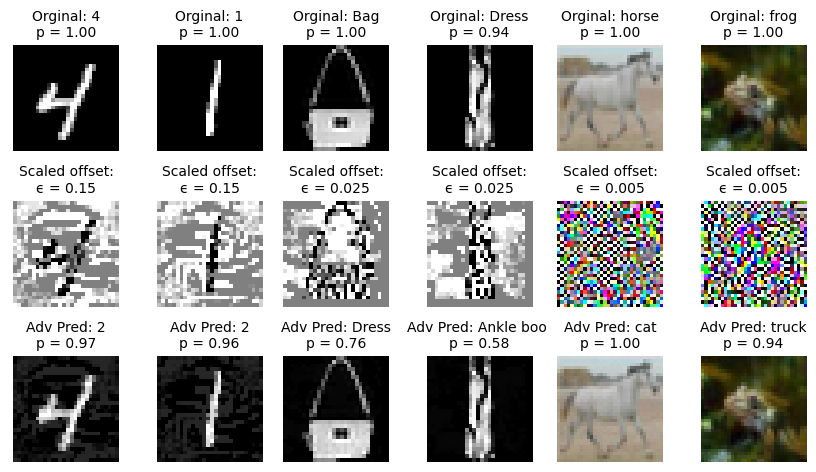
\includegraphics[width=\textwidth]{plots/adv_ex.png}
    \caption{Representative attacks on LeNet, FMNIST, and ResNet-20.}
    \label{fig:adv_ex}
\end{figure}

We observed that the larger and more complicated a model, the more susceptible it is to adversarial attack. 
LeNet5 being a notably small and simple model by contemporary standards, showed remarkable robustness and required attacks well within perceptible levels ($\epsilon \approx 0.3$) before the tested FW methods could reliably produce adversarial examples. While ResNet and FMNIST model can be reliably attacked with $\epsilon$ above $0.07$ and $0.05$ respectively (see Figure \ref{fig:eps}).

\subsection{$\epsilon$ Choice}
Our three different models where retrained on datasets with differing image scales. To allow for comparison of the sensitivity of each model to attacks with different $\epsilon$, at each iteration we normalize to ensure images $x_0$ have mean $0.5$ and variance $1$ to ensure equal relative perturbation of the same $\epsilon$ on all three models. 

\begin{figure}[H]
    \centering
    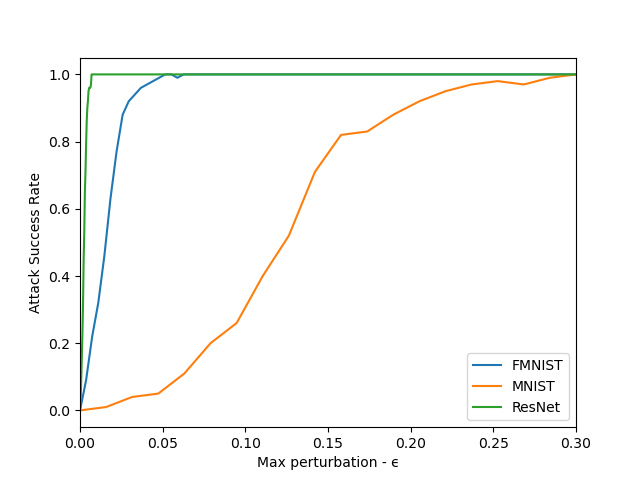
\includegraphics[width=0.7\textwidth]{plots/eps_choice.png}
    \caption{Effect of $\epsilon$ on attack success for untargeted FW for each dataset with $L_\infty$ constraint.}
    \label{fig:eps}
\end{figure}

As figure \ref{fig:converge-compare} shows, the different models have vastly different sensitivities to adversarial attacks. LeNet is the most robust of the three requiring large maximum perturbations for reliable attacks. The larger, more complex models can be reliably attacked with imperceptible examples in the case of ResNet or borderline perceptible in the case of the FMNIST model. Representative attacks are shown in figure 2.

\subsection{Targeted vs. Untargeted Attacks}
We implemented both untargeted and targeted attacks, requiring defining a custom loss function for the pre-trained models. where $f(x) = -\ell(x, y)$ for untargeted attacks, and $f(x) = \ell(x, y_\text{adv})$ where $y$ is the true label and $y_\text{adv}$ the adversarial target class chosen at random to be any class other than $y$. We find, unsurprisingly, that targeted attacks are invariably a more challenging problem, resulting in lower success rates and higher average iterations for all variants and datasets.

For example, attacks on a set of $100$ examples with ResNet-20 and $\epsilon = 0.005$ with normal FW algorithm using decaying rule, achieved a success rate of $0.93$ requiring $5.44$ iterations on average in the untargeted case, but a success rate of $0.63$ and $13.26$ iterations in the targeted case.

\subsection{$L_\infty$ vs $L_2$ Constraints}
We implement attacks Linear Minimization oracles to enable both $L_\infty$ and $L_2$ constrained attacks. 
Choices of $\epsilon$ for the two norms are clearly not comparable as $L_\infty$ is concerned by the maximum perturbation a pixel is perturbed by, doing nothing to disincentives most if not all pixels from being perturbed, where $L_2$ constrains the sum of squares of perturbations. 

\begin{figure}[H]
    \centering
    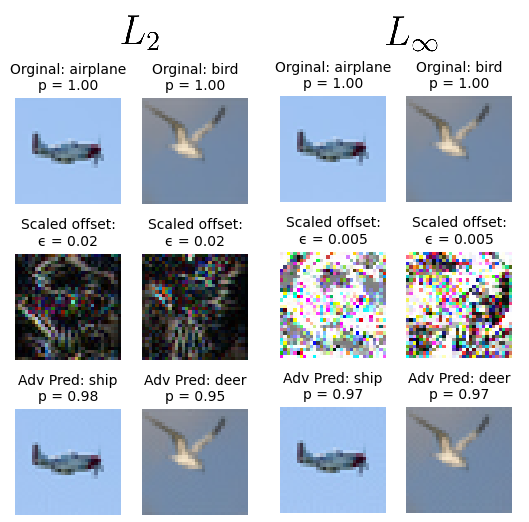
\includegraphics[width=0.6\textwidth]{plots/norm.png}
    \caption{Effect of constraint norm on magnitude of perturbations.}
    \label{fig:norm}
\end{figure}

To compare the resulting adversarial examples generated by attacks I chose $\epsilon$ values that gave approximately the same attack success rate of about $62\%$ on CIFAR-10 ($\epsilon_\infty = 0.005, \epsilon_2 = 0.02$) and compare the $L1$ norm of the generated perturbations. In order to get the same success rate we expected see that $L2$ constrained attacks are more efficient at producing attacks, with an average $L1$ of $6.84$ ($\sigma = 0.69$) where $L_\infty$ constrained attacks created attacks with average perturbation $L_1$ of $10.5$. However, we note that both cases produced attacks below with marginal perceptibility with $L_2$ attacks having an average $L_\infty$ of $0.013$ and it being difficult to think of applications were this efficiency is worth the trade off.  We also observe, that it takes longer on average for $L_2$ constrained attacks to converge. Normal FW took 12.71 in $L_\infty$ case and $13.2$ for the $L_2$ case. From our testing we did not see any pirticular varient disproportionately affected by the choice of norm.
We visualize the magnitude of attacks made by the attacks using the different constraints in figure \ref{fig:norm}. 


\subsection{Step-size}
The methods for step-size were implemented as follows: 
%Lipschitz constant-based (fixed) step-size, where the step-size is determined using the Lipschitz constant \(L\) with \(\gamma_t = \frac{1}{L}\); 
 Decaying step-size, where the step-size decreases over time according to $\gamma_t = \frac{2}{t + 2}$; 
exact line-searching, which solves the optimization problem $\text{argmin}_{\gamma} f(x + \gamma d_t)$ where $\gamma \in (0,\gamma_t^\text{max}]$; 
and Armijo-rule search, which defines stepsizes for each iteration $k$: $\gamma_t = \delta^k \gamma_t^\text{max}$ and tests for satisfactory decrease  in the objective relative to the step-size as captured by the the Armijo condition $f(x + \gamma_t d_t) \leq f(x) + \beta \gamma_t \langle\nabla f(x), d_t\langle$, where $\delta \in (0,1)$ and $\beta \in (0, 0.5)$ are fixed parameters that controll the step-size decrease at each iteration, and the desired improvement respectively. This method is well suited to this application, as it aims to provide the convergence benifits provided by adaptive step-sizes while drastically reducing queries to the loss function which is expensive in the context of adversarial attacks.

We found the application of line-searching techniques to be marginally benifit attack success rate, and appreciably decrease iterations required to converge. 
On a consumer grade machine and without parallizing model queries, we show the results of the three different algorithims. Where exact-LS tests 50 equally spaced stepsizes $\gamma_t \in (0, \gamma_t^\text{max}]$, and Armijo rule used parameters we found to perform well through experimentation: $\gamma = 0.5, \beta = 0.5$.

\begin{table}[H]
\centering
\begin{tabular}{lccc}
\toprule
\textbf{Step Rule} & \textbf{ASR (\%)} & \textbf{Avg. Iters} & \textbf{Attacks/Second} \\
\midrule
Decay  & 62.4 & 13.52 & 4.5 \\
Armijo & 63.6 & 13.13 & 2.5 \\
Exact-LS & 63.8 & 12.98 & 0.34 \\
\bottomrule
\end{tabular}
\caption{Attack Success Rate (ASR) for PFW and Attacks/Second for Different Step Rules}
\label{table:asr_step_rules}
\end{table}

\subsection{Momentum}

Momentum proved highly effective at reducing the number of iterations required for convergence with minimal effect attack success rate. On a test of $1000$ examples from CIFAR-10. Normal FW provided an ASR of $88.7\%$ with average of $11.39$ iterations. FW with momentum ($\beta = 0.8$) achieved $89.5\%$ ASR and $8.47$ mean iterations, indicating a significant improvement in convergence (see Figure \ref{fig:momentum}). This is seen to outperform all other varients with the same parameters, achieving appreciably better ASR and mean convergence time.

\begin{figure}[H]
    \centering
    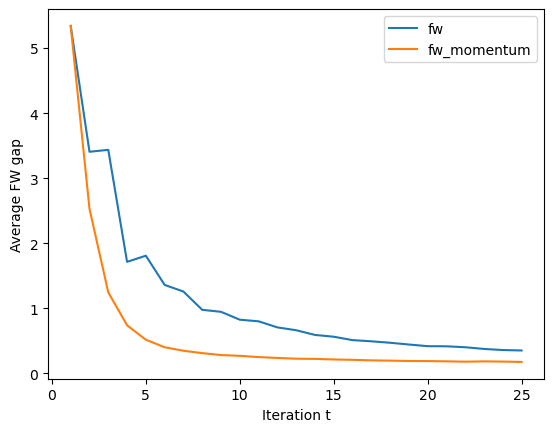
\includegraphics[width=0.7\textwidth]{plots/momentum.png}
    \caption{Comparison of $g_t^\text{FW}$ of FW and momentum varient targeted attacks on ResNet-20 with $\epsilon = 0.007$ and $\beta = 0.8, N = 1000$.}
    \label{fig:momentum}
\end{figure}

\subsection{Variants}

% DUMMY VALUES NEED TO BE CHANGED
\begin{table}[H]
    \centering
    \resizebox{\textwidth}{!}{
    \begin{tabular}{@{}lcccccccc@{}}
        \toprule
        \multirow{3}{*}{\textbf{Algorithm}} & \multicolumn{2}{c}{\textbf{MNIST}} & \multicolumn{2}{c}{\textbf{F-MNIST}} & \multicolumn{2}{c}{\textbf{CIFAR-10}} \\
        & \multicolumn{2}{c}{$\epsilon=0.16$} & \multicolumn{2}{c}{$\epsilon=0.04$} & \multicolumn{2}{c}{$\epsilon=0.005$} \\
        \cmidrule(lr){2-3} \cmidrule(lr){4-5} \cmidrule(lr){6-7}
        & \textbf{ASR (\%)} & \textbf{Avg Iter} & \textbf{ASR (\%)} & \textbf{Avg Iter} & \textbf{ASR (\%)} & \textbf{Avg Iter} \\
        \midrule
        FW & 62.2 & 50 & 67.6 & 16.35 & 66.0 & 12.71 \\
        AFW & 62.2 & 45 & 67.8 & 16.35 & 65.0 & 12.8 \\
        PFW & 62.2 & 47 & 62.2 & 17.03 & 64.0 & 13.48 \\
        \bottomrule
    \end{tabular}
    }
    \caption{Attack Success Rate (ASR) and Average Iterations of Frank-Wolfe Algorithm and Variants for Targeted Adversarial Attacks on 1000 Examples from Three Datasets with $20$ maximum iterations and decaying step-size rule.}
	\label{table:varients}
\end{table}
We note that $\epsilon$ values were chosen to create a difficult optimization problem that highlighted differences in convergence between algorithms, and $\epsilon$ could have been easily chosen to ensure $100\%$ ASR on all datasets.

We observe that the difficulty of the optimization problem, as influenced by the choice of dataset to attack, $\epsilon$ choice, and performing either targeted or untargeted attacks will effect the number of Away Steps taken by AFW. Targeted attacks on CIFAR-10 as described in table \ref{table:varients}. For Both attacks on LeNet5 and FMNIST model, AFW was never seen to take an away step. However, when attacking ResNet-20, it is seen to have taken Away Steps $17.1\%$ of the time. As it takes majority FW steps, the convergence of AFW is seen to closely follow that of normal FW (see Figure \ref{fig:converge-compare}).

%REPLACE WITH FINAL RESULTS
\begin{figure}[H]
    \centering
    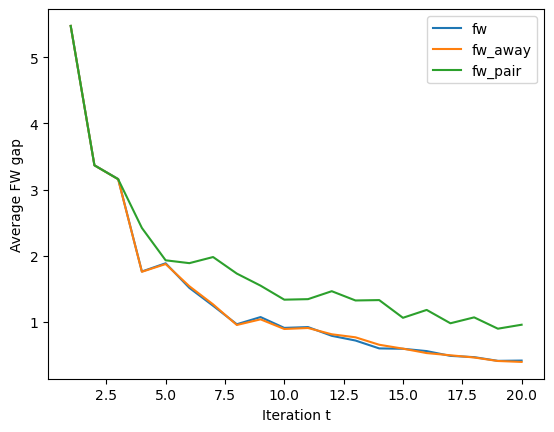
\includegraphics[width=0.7\textwidth]{plots/mdl_compare_avg_FWgap_by_iter.png}
    \caption{Average $g^\text{FW}_t$ for each Algorithm by Iteration for Targeted Attacks on ResNet-20 (CIFAR-10) with decaying rule and $\epsilon = 0.005$.}
    \label{fig:converge-compare}
\end{figure}

We observe that this application does not favor the use of PFW. Which we attribute to the lack of line-searching, which we found to be inappropriate for the non-convex application. Analysis of the away costs at each iteration showed that $g_t^\text{A}$ is often negative, indicating that it is still a good atom in the active set $S_t$. In the absence of line-searching, PFW with decaying rule frequently will over minimize, or even drop the contribution $v_t$ to $x_t$ harming convergence and attack success rate. We observe that the use of line-searching harms the  of PFW less so than the other two algorithms, making their performance more comparable. But still suffers form the aforementioned problems associated with non-convexity and line searching.



\section{Convergence Analysis}
% Proof adaptaed from https://arxiv.org/pdf/1607.00345
% Convergence Rate of Frank-Wolfe for Non-Convex Objectives (Lacoste-Julien 2016)
The convergence of the FW algorithms in this application is complicated by the non-convexity of the DNN objective function.
We reproduce a proof from Lacoste-Julien \cite{fw-noncovex} for the sub-linear convergance of FW in the non-convex case. The sublinear rate of the momentum varient has an elegant proof from Chen et. al. \cite{attacks}. We comment on the intuition behind the two varients (AFW and PFW) acheiving linear rates in the convex case.
For the following proof we assume that $f$ has $L$-Lipschitz continuous gradient on $\mathcal{M}$. This is to say that 
$$ f(y) \leq f(x) + \nabla f(x)^T (y-x) + \frac{L}{2}||y-x||_2^2$$.
This has been shown to be a reasonable assumption for DNN. %Santurkar et al. 2018, mentioned in attacks.pdf
Lipshitz continuous gradient gives us bound on curvature constant $C_f$ % (eq5) https://arxiv.org/pdf/1607.00345
Where $C_f$ is the smallest constant such that 
We additionally require that our constraint space $\mathcal{M}$ is convex and compact with diameter $D$. Satisfying $||x-y||_2 \leq D$ for $x,y \in \mathcal{M}$. This is trivially satisfied in the application of adversarial attacks, considering the definition of $\mathcal{M}$. 
Where Chen et al. 2020 used this strategy to prove the convergence of FW with momentum. We the result holds for normal FW. 
At each iteration since $s_t \in \mathcal{M}$, we get that $||\nabla f(x_t) - s_t||_2$

\subsection{Frank-Wolfe}
\subsection{Pairwise Frank-Wolfe}
\subsection{Away-Step Frank-Wolfe}

\bibliographystyle{plain}  % Choose a bibliography style
\bibliography{ref}
\end{document}